\documentclass{beamer}

\usepackage{changepage}
\usepackage{subcaption}
\usepackage{sidecap}

\setbeamertemplate{caption}{\insertcaption}

\title{Dubins and Reeds–Shepp paths}
\date{}%\date{January 2022}
\author{Benjamin Loison}

\addtobeamertemplate{navigation symbols}{}
{
    \usebeamerfont{footline}
    \usebeamercolor[fg]{footline}
    \hspace{1em}
    \insertframenumber/\inserttotalframenumber
}

\setbeamercolor{footline}{fg=blue}
\setbeamerfont{footline}{series=\bfseries}
% could remove some navigation symbols

\begin{document}

\frame{\titlepage}

\begin{frame}
\frametitle{Table of contents}
\tableofcontents
\end{frame}

\section{Dubins' paths}

\begin{frame}

\frametitle{Introduction}

\begin{figure}
\centering
  \centering
  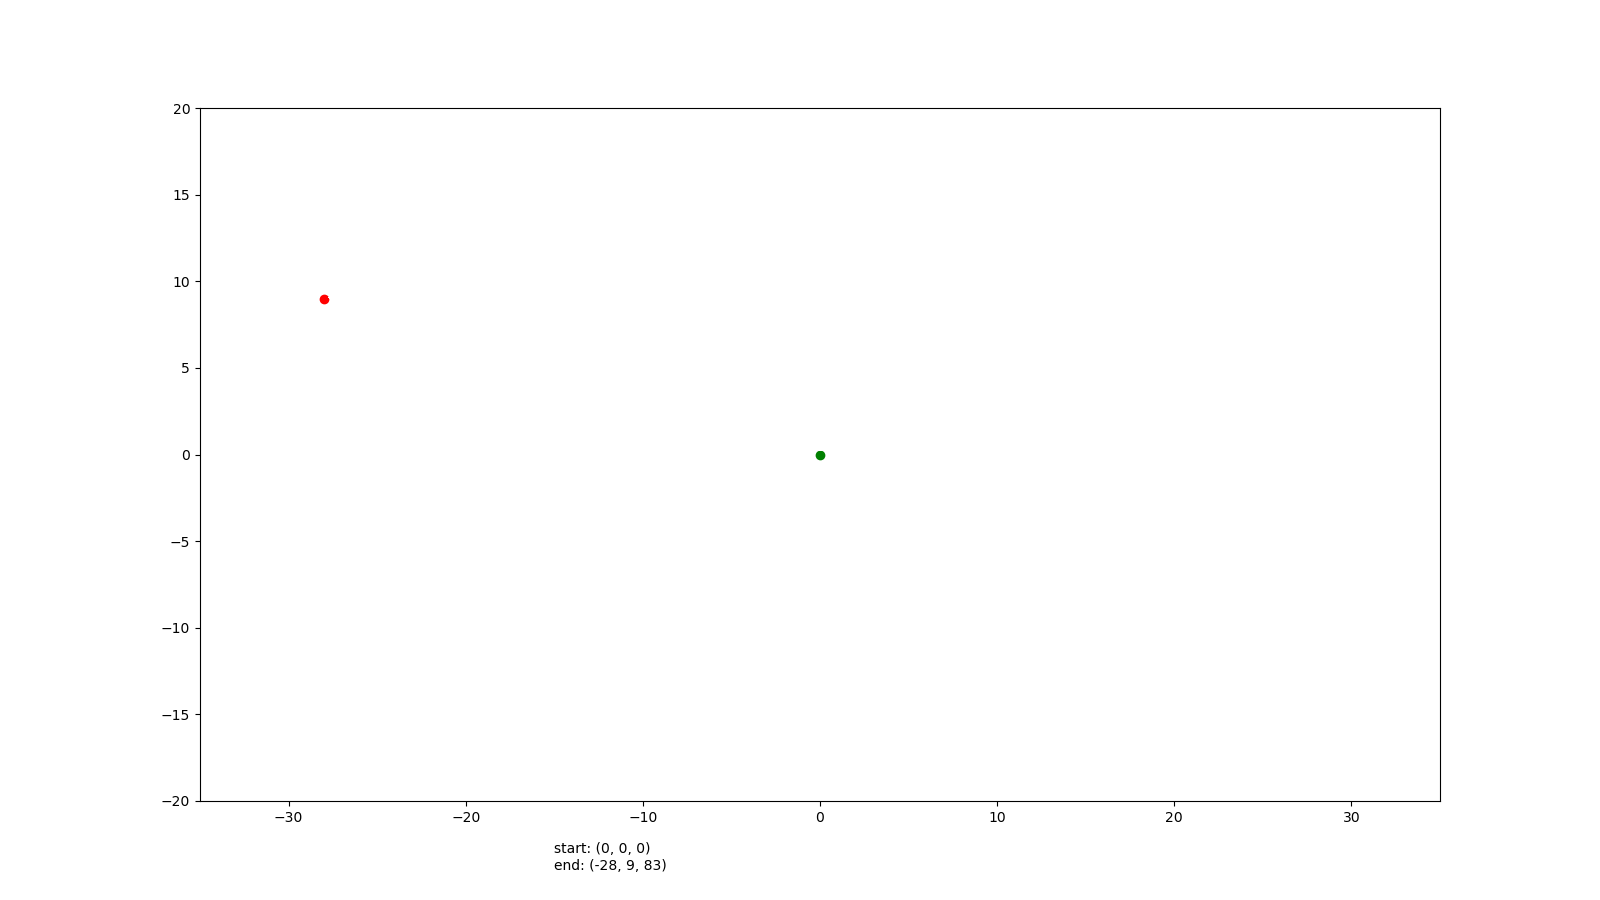
\includegraphics[width=1.1\linewidth]{Illustrations/human.png}
  \caption{The shortest path in the case of a human being}
  \label{fig:sub1}
\end{figure}
\end{frame}

\begin{frame}

\frametitle{Introduction}

\begin{figure}
\centering
  \centering
  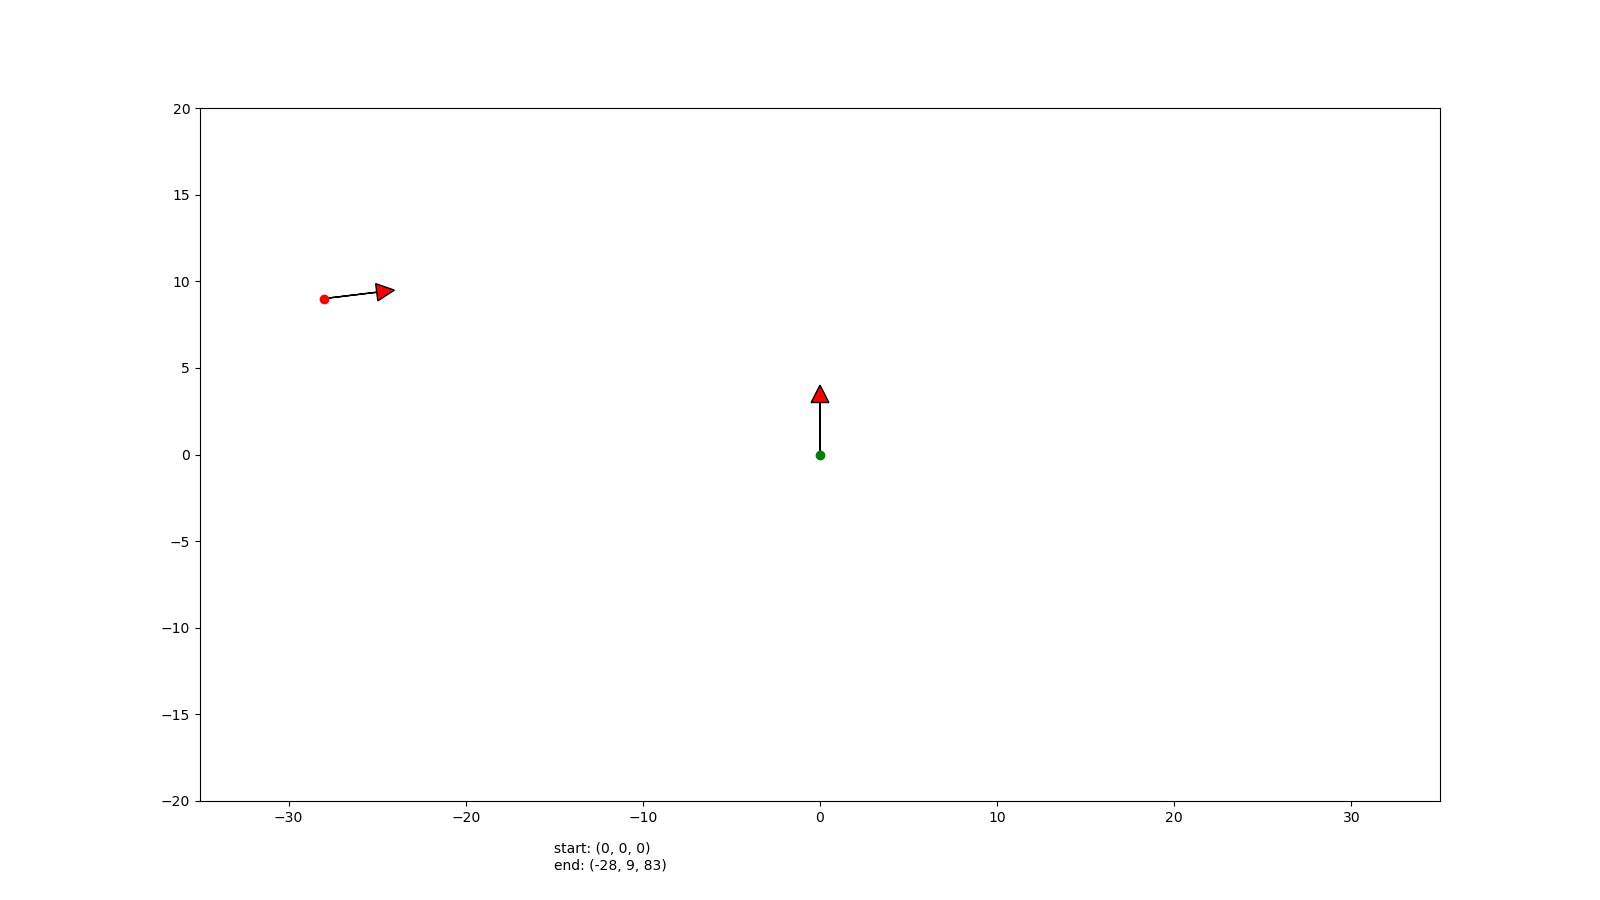
\includegraphics[width=1.1\linewidth]{Illustrations/humanOriented.png}
  \caption{A shortest path in the case of an oriented human being}
  \label{fig:sub1}
\end{figure}
\end{frame}

\begin{frame}

\frametitle{Introduction}

\begin{figure}
\centering
  \centering
  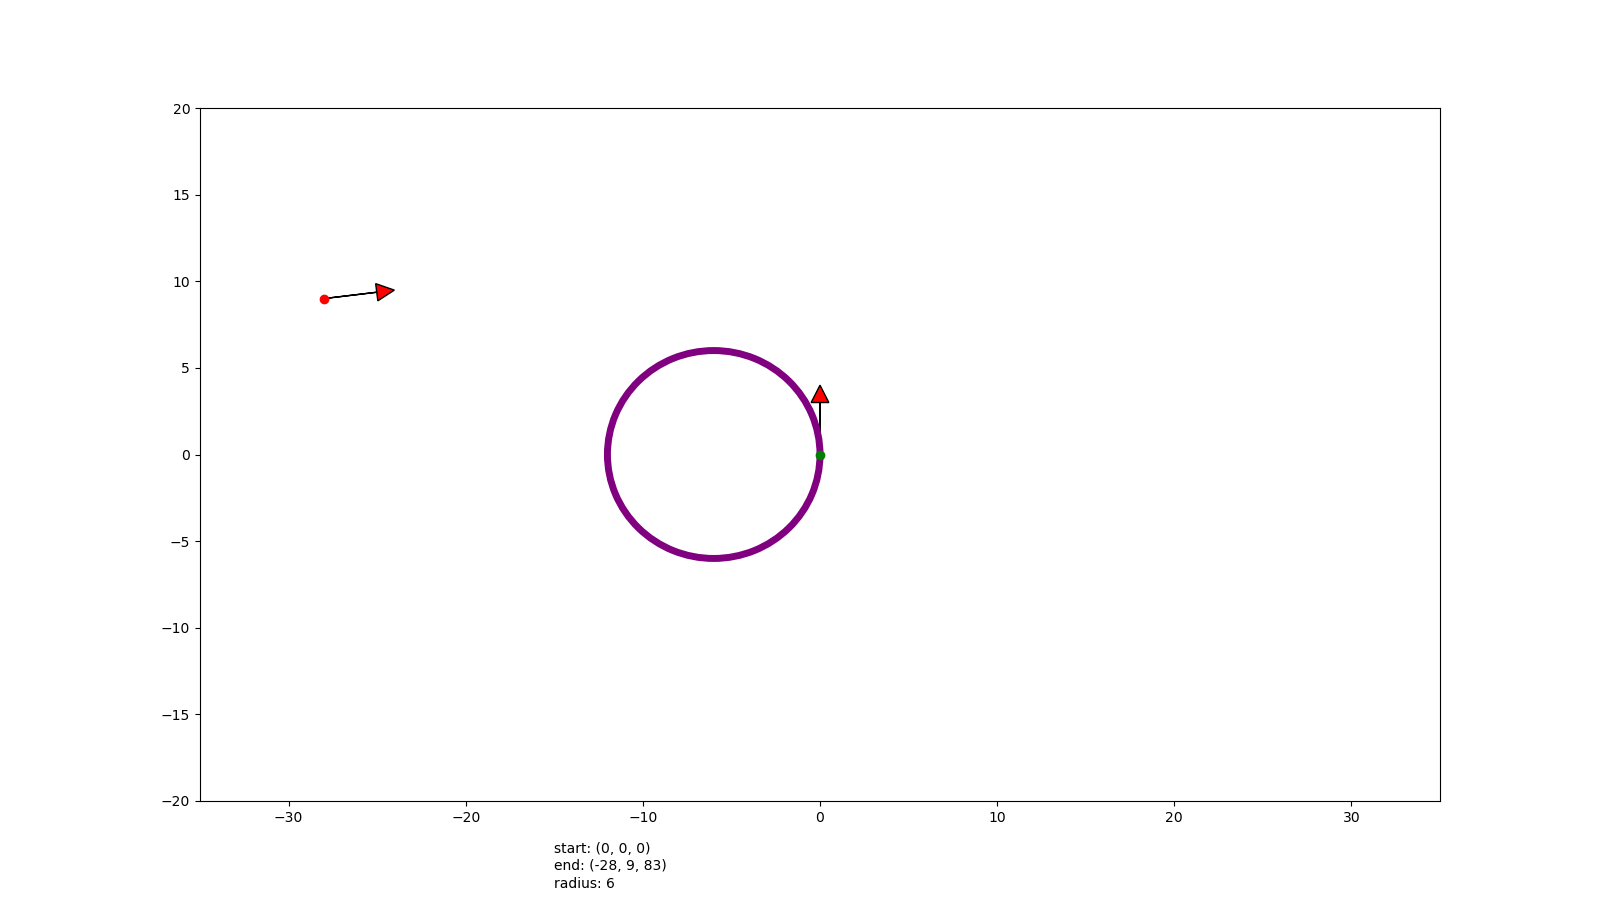
\includegraphics[width=1.1\linewidth]{Illustrations/robotMinimumCircle.png}
  \caption{Robot's minimal turning circle}
  \label{fig:sub1}
\end{figure}
\end{frame}

\begin{frame}

\frametitle{Dubins' paths}

\begin{figure}
\centering
  \centering
  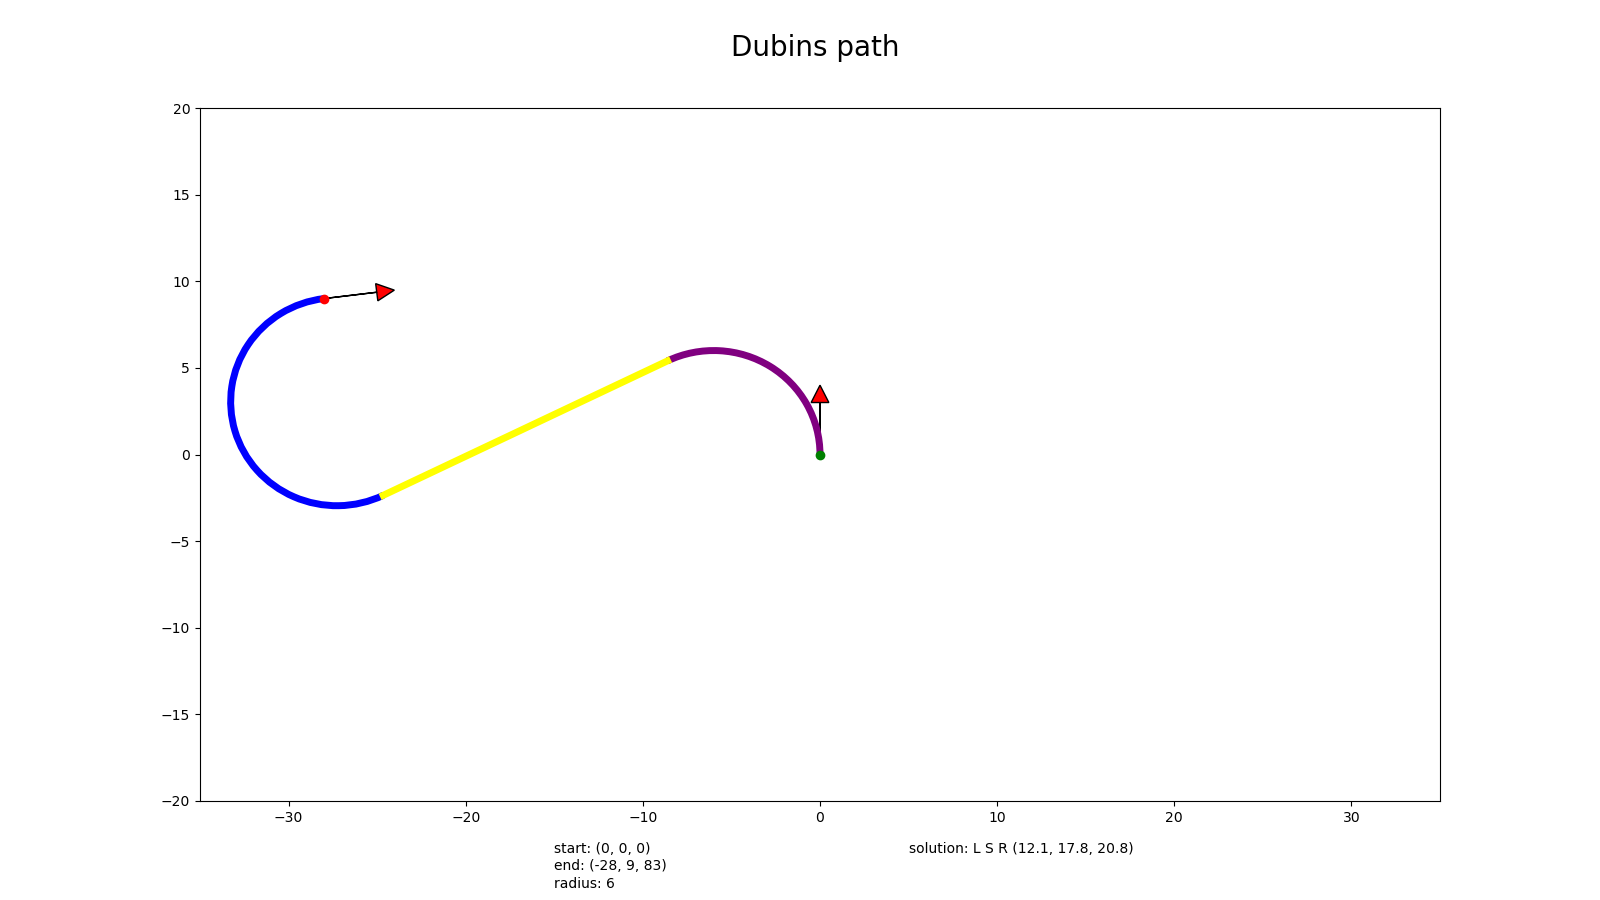
\includegraphics[width=1.1\linewidth]{Illustrations/002.png}
  \caption{Dubins' path descriebing a shortest path}
  \label{fig:sub1}
\end{figure}
\end{frame}

\begin{frame}

\frametitle{Dubins' paths}

\vspace{0.5cm}

\begin{table}[h]
    \begin{subtable}[h]{0.45\textwidth}
        \centering
        \begin{tabular}{| c |}
        \textbf{CSC} \\
        \hline \hline
        RSR \\
        LSL \\
        LSR \\
        RSL
       \end{tabular}
				\caption{All combinaisons of \textbf{CSC} paths}
    \end{subtable}
    \hfill
        \begin{subtable}[h]{0.45\textwidth}
        \centering
        \begin{tabular}{| c |}
        \textbf{CCC} \\
        \hline \hline
        RLR \\
        LRL
       \end{tabular}
			\caption{All combinaisons of \textbf{CCC} paths}
    \end{subtable}
\end{table}

	\vspace*{1cm}

	C: means "curve" (i.e. turning left or right)\\
	S: means "straight"\\\\
	
	R: means "right" (i.e. turning right)\\
	L: means "left" (i.e. turning left)

\end{frame}

\begin{frame}

\frametitle{Dubins' paths}

\begin{figure}
\centering
  \centering
  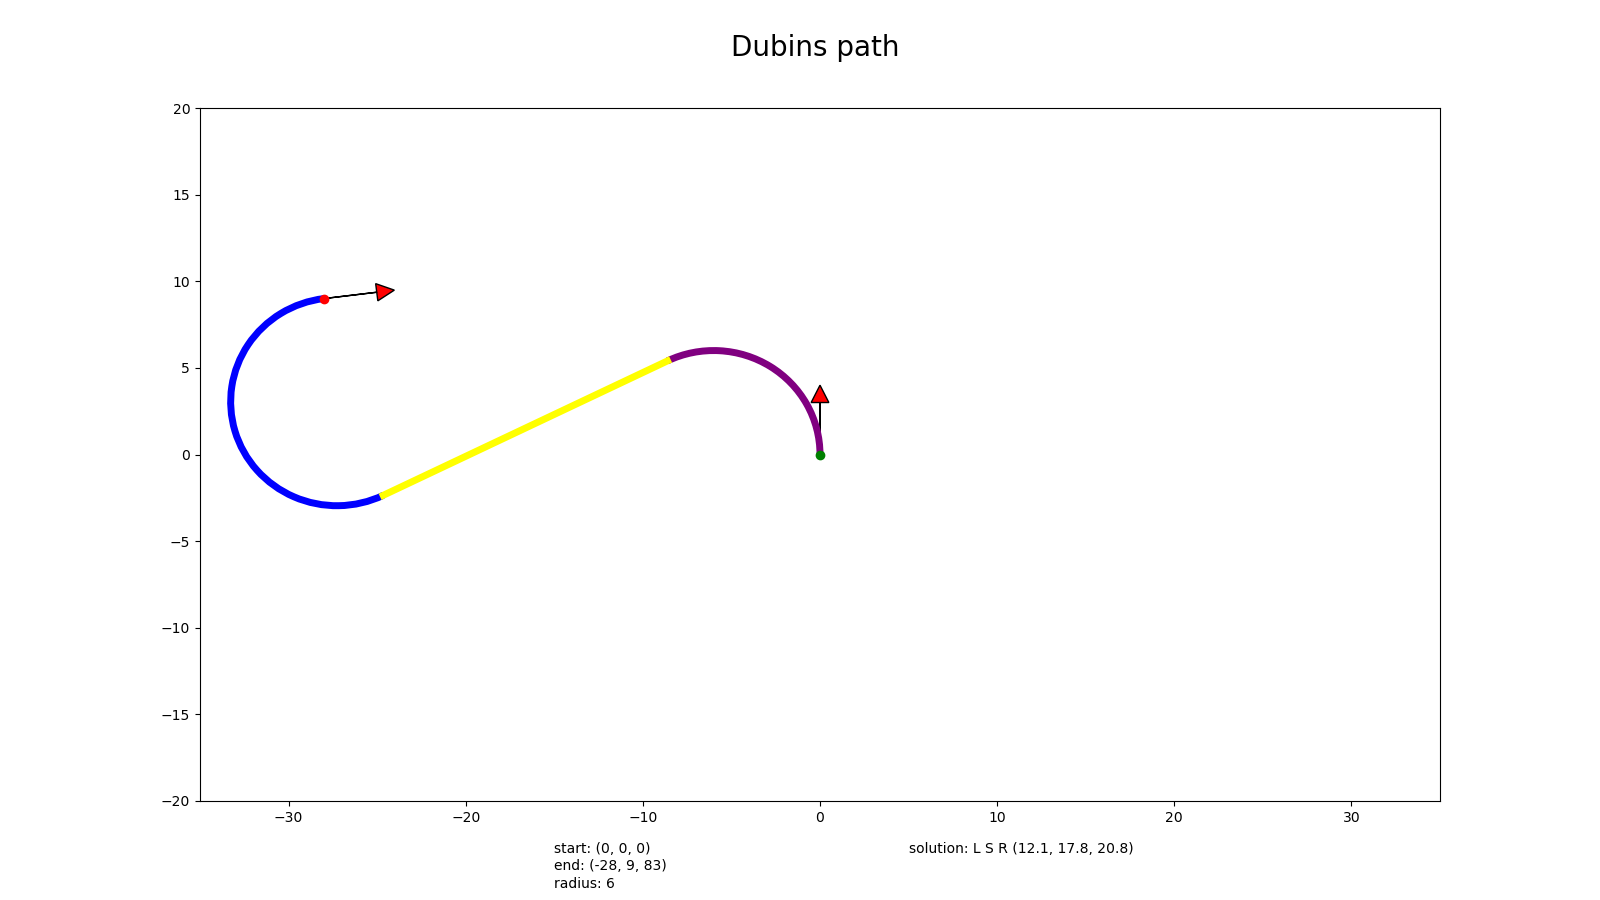
\includegraphics[width=1.1\linewidth]{Illustrations/002.png}
  \caption{Dubins' path LSR descriebing the shortest path}
  \label{fig:sub1}
\end{figure}
\end{frame}

\section{Implementation details}

\begin{frame}


\frametitle{Implementation details}

\begin{enumerate}
	\pause
	\item Constant complexity
	\pause
	\item Use of a table on angles
	\pause
	\item Outer and inner tangents
	\begin{figure}
	\centering
		\centering
		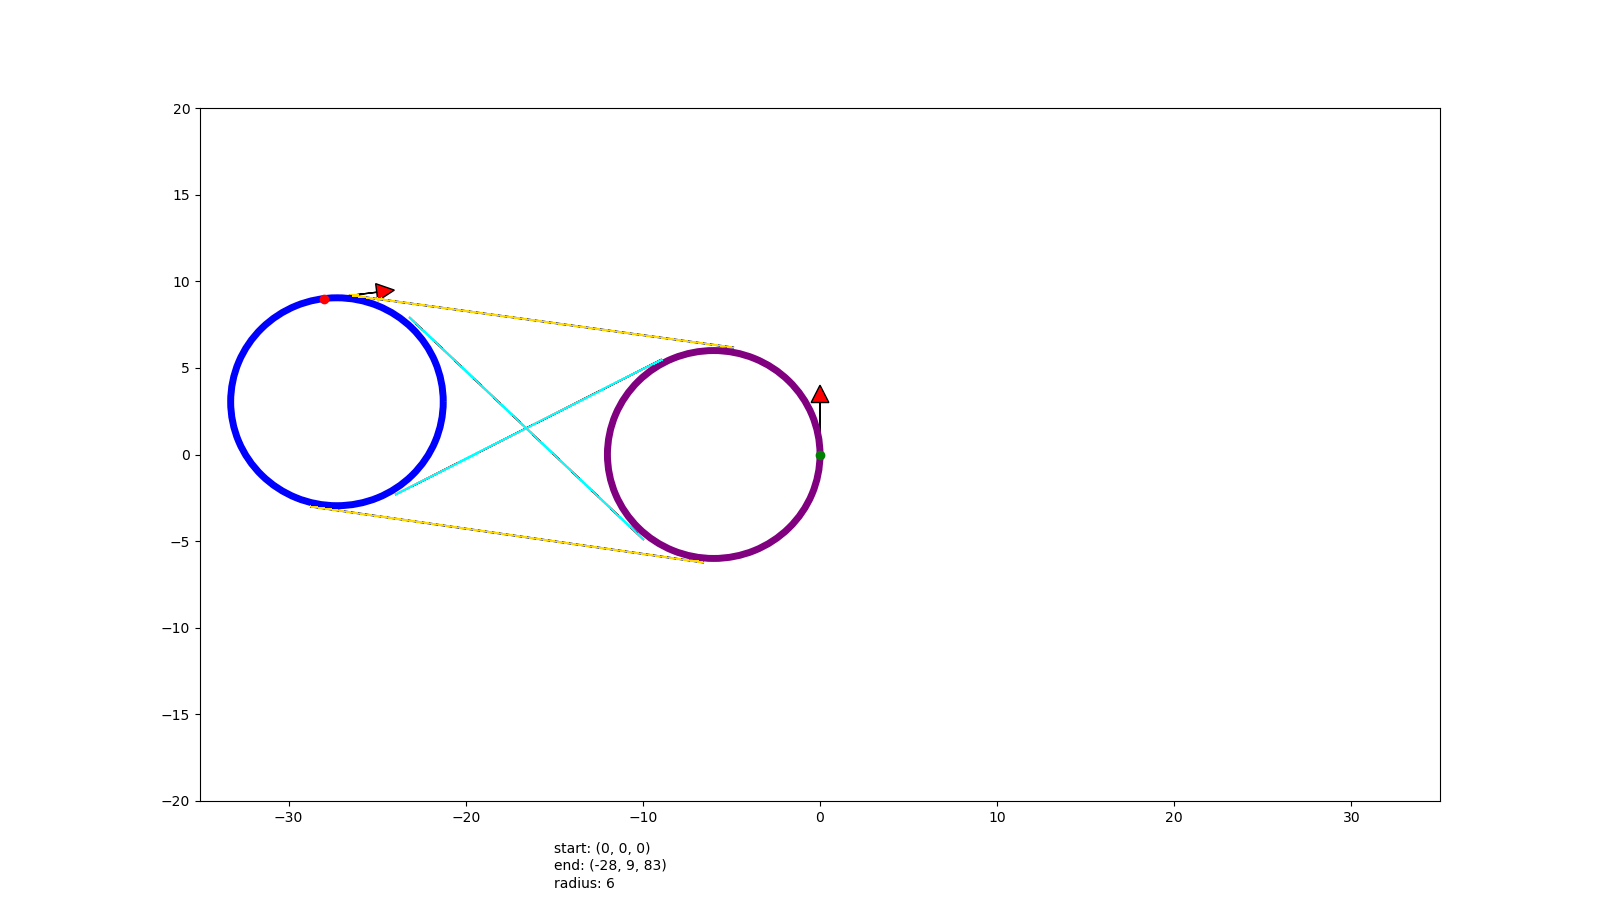
\includegraphics[width=\linewidth]{Illustrations/001tangents.png}
		\caption{Same radius internal and external circles tangents}%Same radius circles for departure and arrival oriented positions}
		\label{fig:sub1}
	\end{figure}
\end{enumerate}

\end{frame}

\begin{frame}


\frametitle{Implementation details}

\begin{itemize}
	\item $\dot{x} =$ cos $\theta$
	\item $\dot{y} =$ sin $\theta$
	\item $\dot{\theta} = \frac{1}{r_{\textt{min\ turning}}}$
\end{itemize}

\begin{itemize}
	\item $x_{new} = x_{prev} + \delta * cos(\theta)$
	\item $y_{new} = y_{prev} + \delta * sin(\theta)$
	\item $\theta_{new} = \theta_{prev} + \frac{\delta}{r_{\textt{min\ turning}}}$
\end{itemize}

With $\delta$ a small value, typically below 0.05.

\end{frame}

\section{Reeds-Shepp paths}

\begin{frame}

\frametitle{Reeds-Shepp paths}

\begin{figure}
\centering
  \centering
  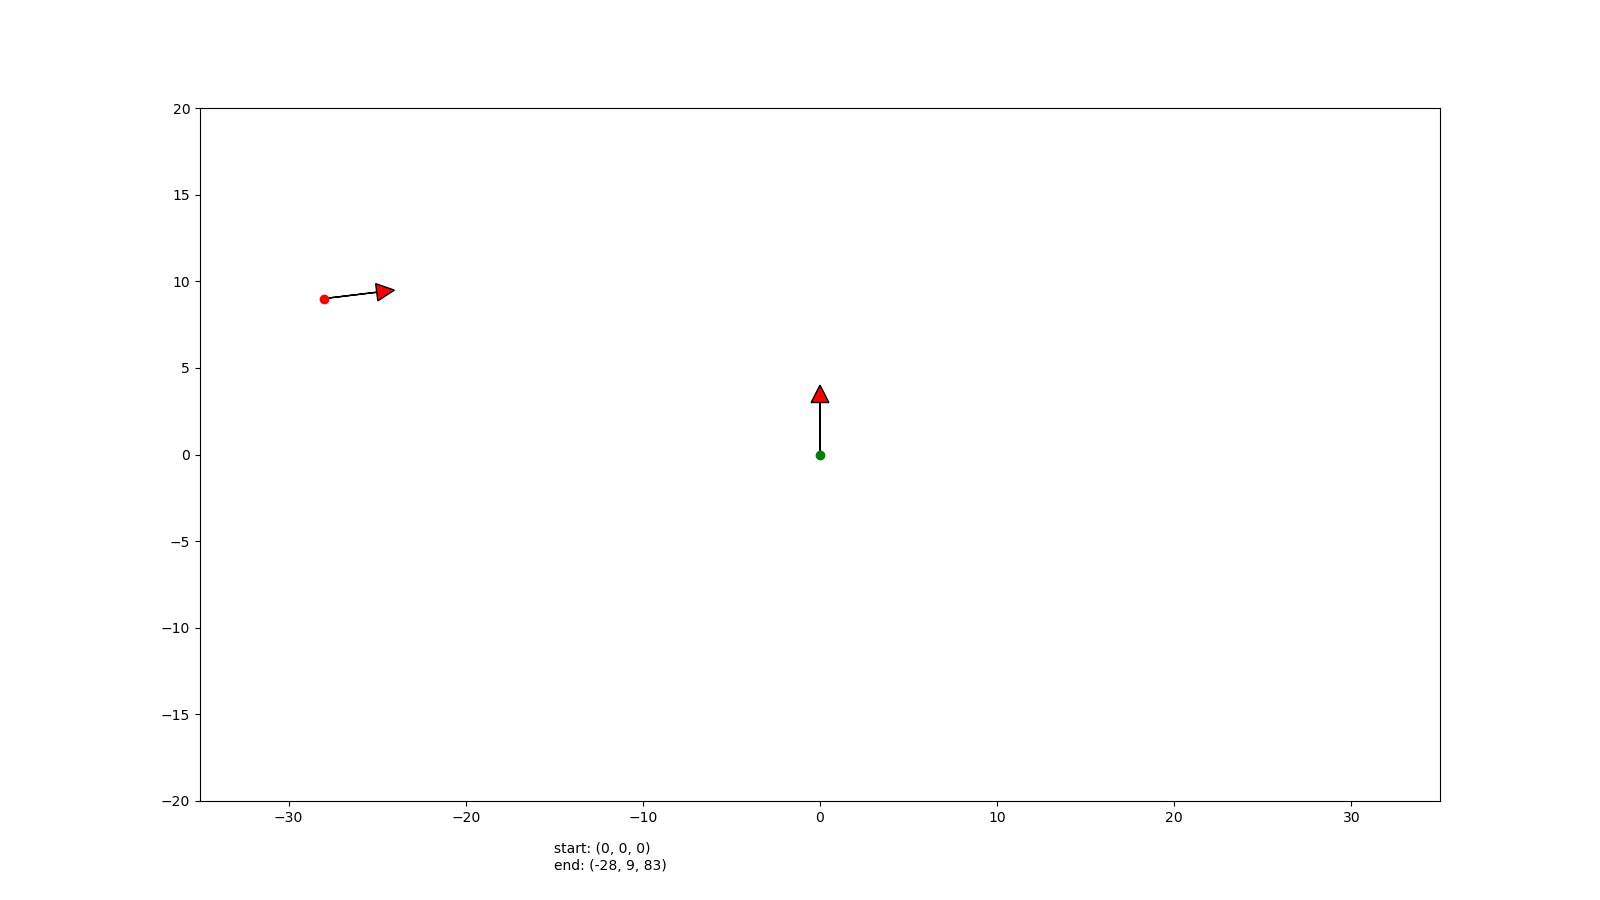
\includegraphics[width=1.1\linewidth]{Illustrations/humanOriented.png}
  \caption{What is a shortest path for a robot able to go backward ?}
  \label{fig:sub1}
\end{figure}
\end{frame}

\begin{frame}

\frametitle{Reeds-Shepp paths}

\begin{figure}
\centering
  \centering
  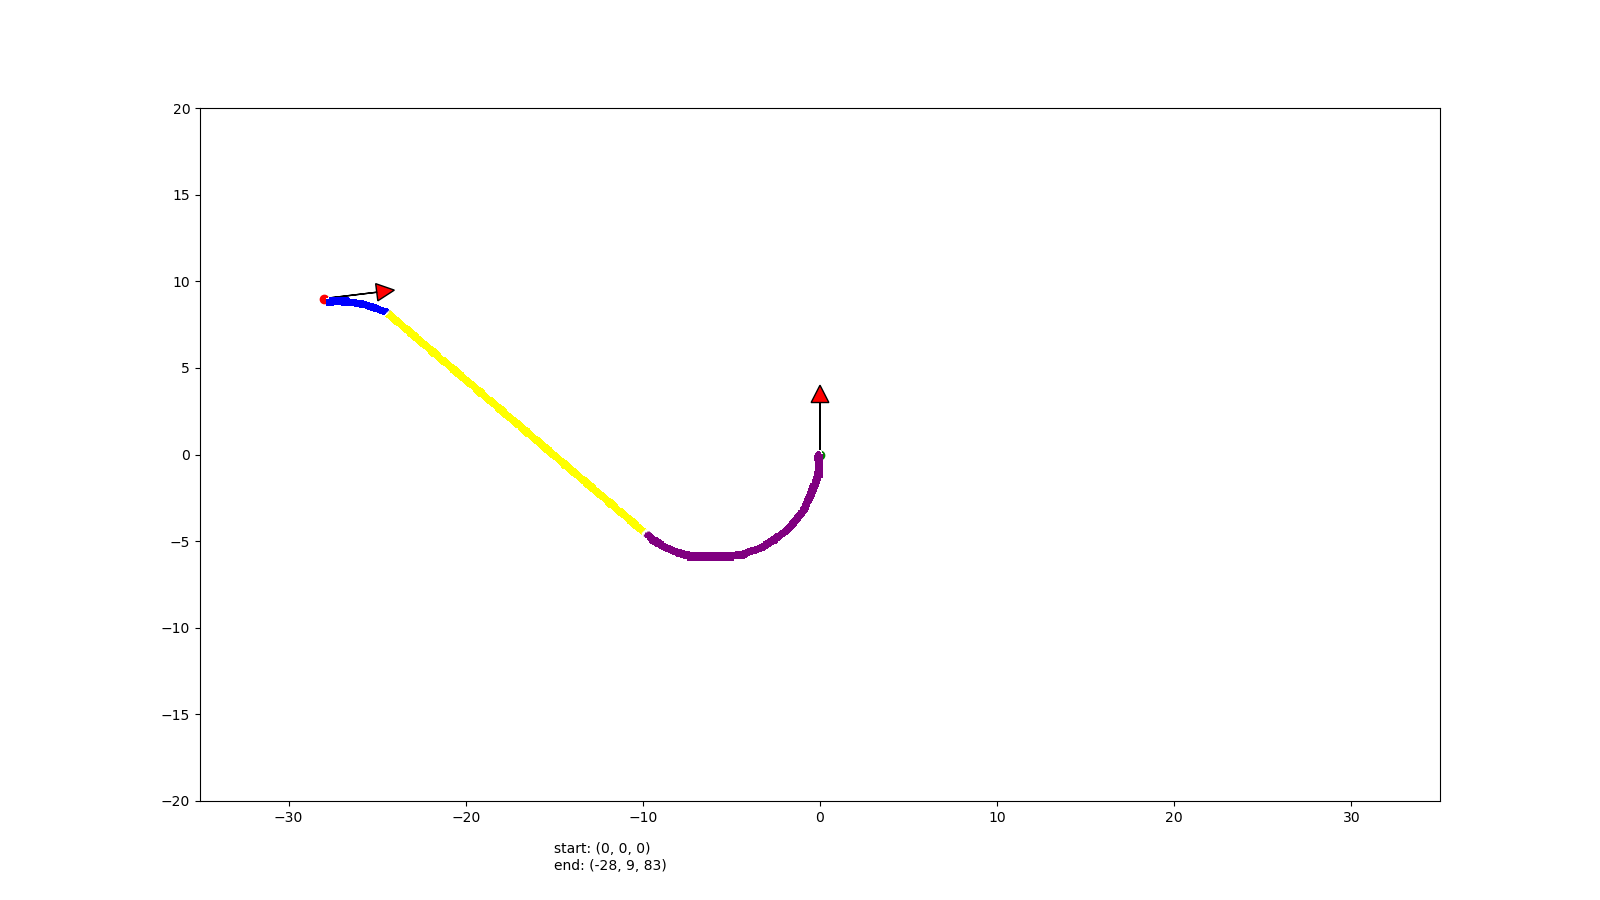
\includegraphics[width=1.1\linewidth]{Illustrations/ReedsSheppBeautiful.png}
  \caption{A shortest Reeds-Shepp path for a robot able to go backward}
  \label{fig:sub1}
\end{figure}
\end{frame}

\begin{frame}

\frametitle{Reeds-Shepp paths}

\begin{figure}
\centering
  \centering
  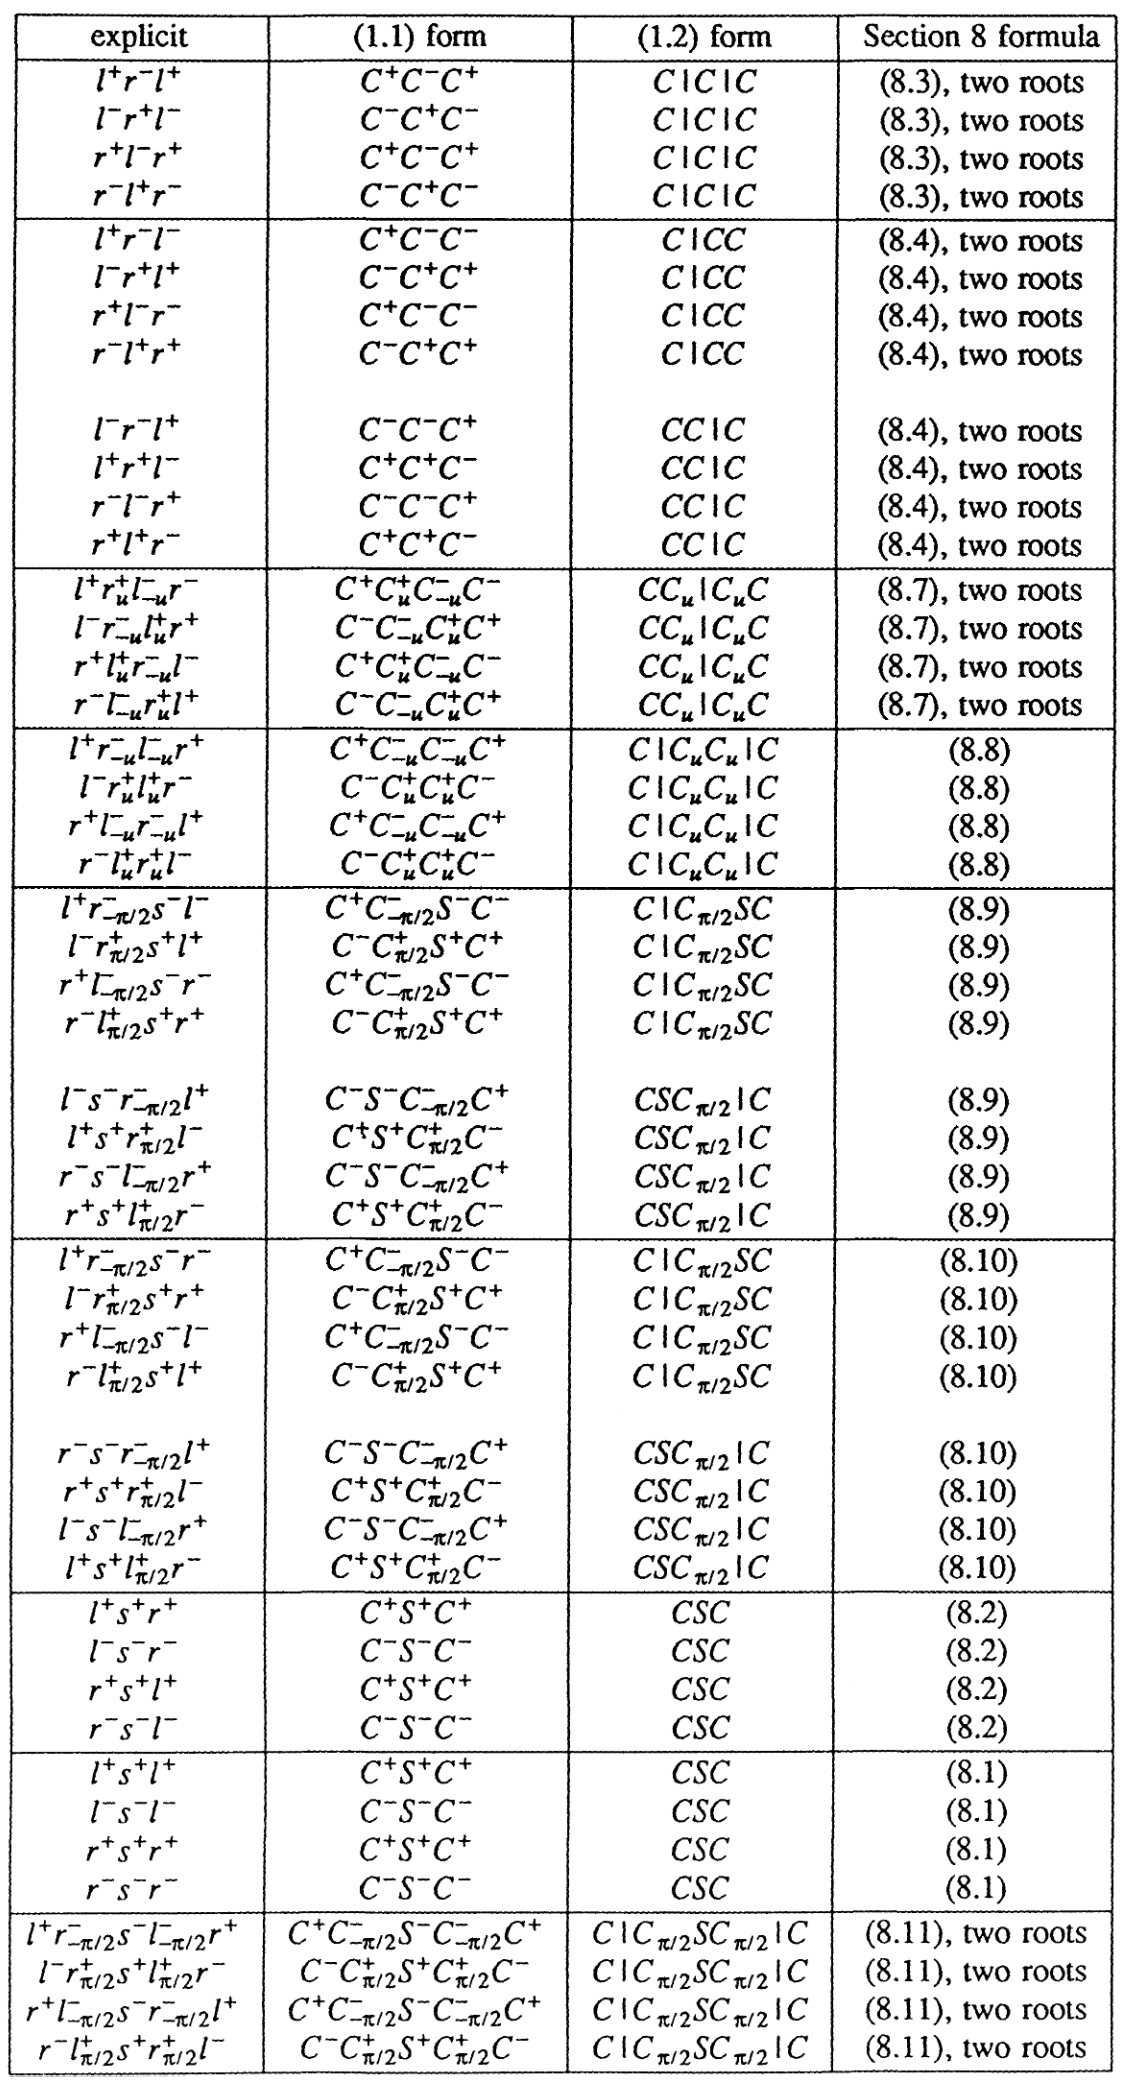
\includegraphics[width=0.4\linewidth]{Illustrations/ReedsSheppPossibilitiesNoTitle.png}
  \caption{All Reeds-Shepp paths}
  \label{fig:sub1}
\end{figure}
\end{frame}

\section{Reeds-Shepp paths simplifications}

\begin{frame}

\frametitle{Reeds-Shepp paths: timeflip simplification}

\begin{figure}
\centering
  \centering
  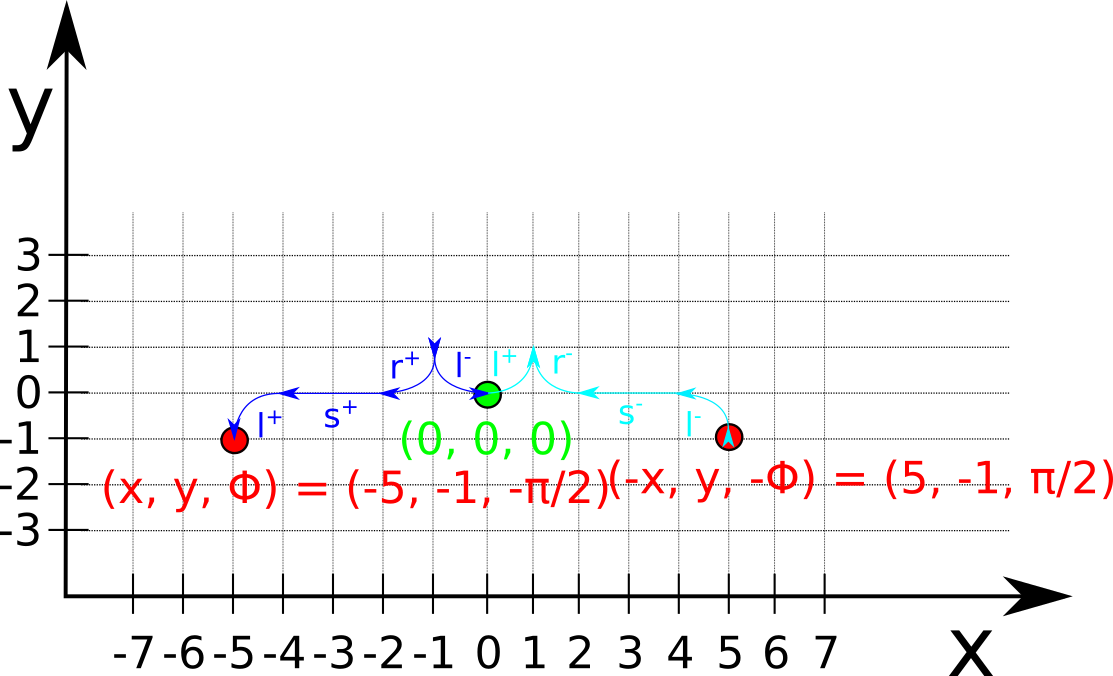
\includegraphics[width=\linewidth]{Illustrations/timeflip.png}
  \caption{Timeflip simplification: $l^-r^+s^+l^+$ goes from the (0, 0, 0) to ($x, y, \phi$) and $l^+r^-s^-l^-$ goes from (0, 0, 0) to ($-x,y,-\phi$)}
  \label{fig:sub1}
\end{figure}
\end{frame}

\begin{frame}

\frametitle{Reeds-Shepp paths: timeflip simplification}

\begin{figure}
\centering
  \centering
  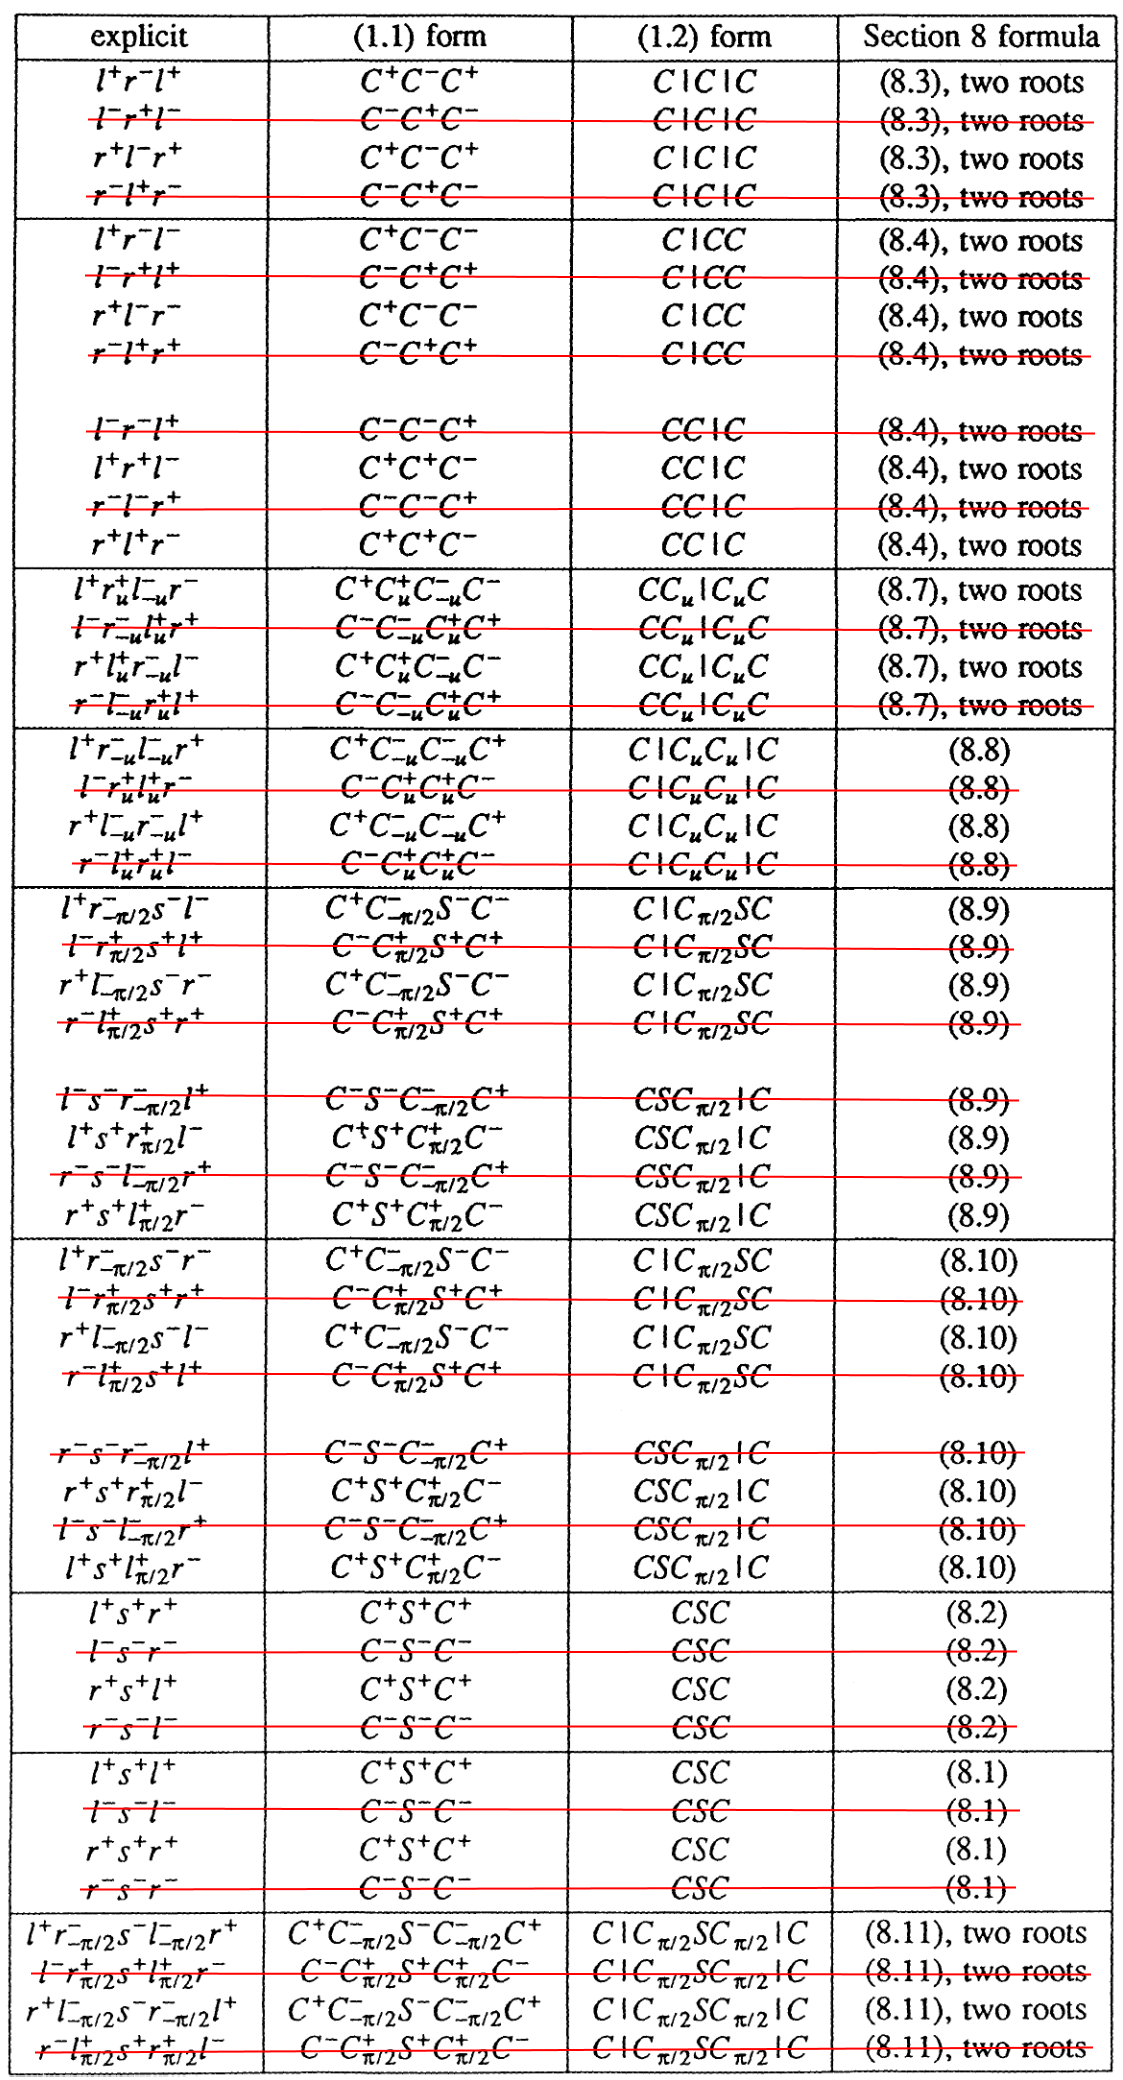
\includegraphics[width=0.4\linewidth]{Illustrations/ReedsSheppPossibilitiesNoTitleNoTimeflip.png}
  \caption{All Reeds-Shepp paths with \textcolor{red}{timeflip} simplification}
  \label{fig:sub1}
\end{figure}
\end{frame}

\begin{frame}

\frametitle{Reeds-Shepp paths: reflect simplification}

\begin{figure}
\centering
  \centering
  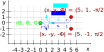
\includegraphics[width=\linewidth]{Illustrations/reflect.png}
  \caption{Reflect simplification: $r^+l^-s^-r^-$ goes from the (0, 0, 0) to ($x, y, \phi$) and $l^+r^-s^-l^-$ goes from (0, 0, 0) to ($x,-y,-\phi$)}
  \label{fig:sub1}
\end{figure}
\end{frame}

\begin{frame}

\frametitle{Reeds-Shepp paths: reflect simplification}

\begin{figure}
\centering
  \centering
  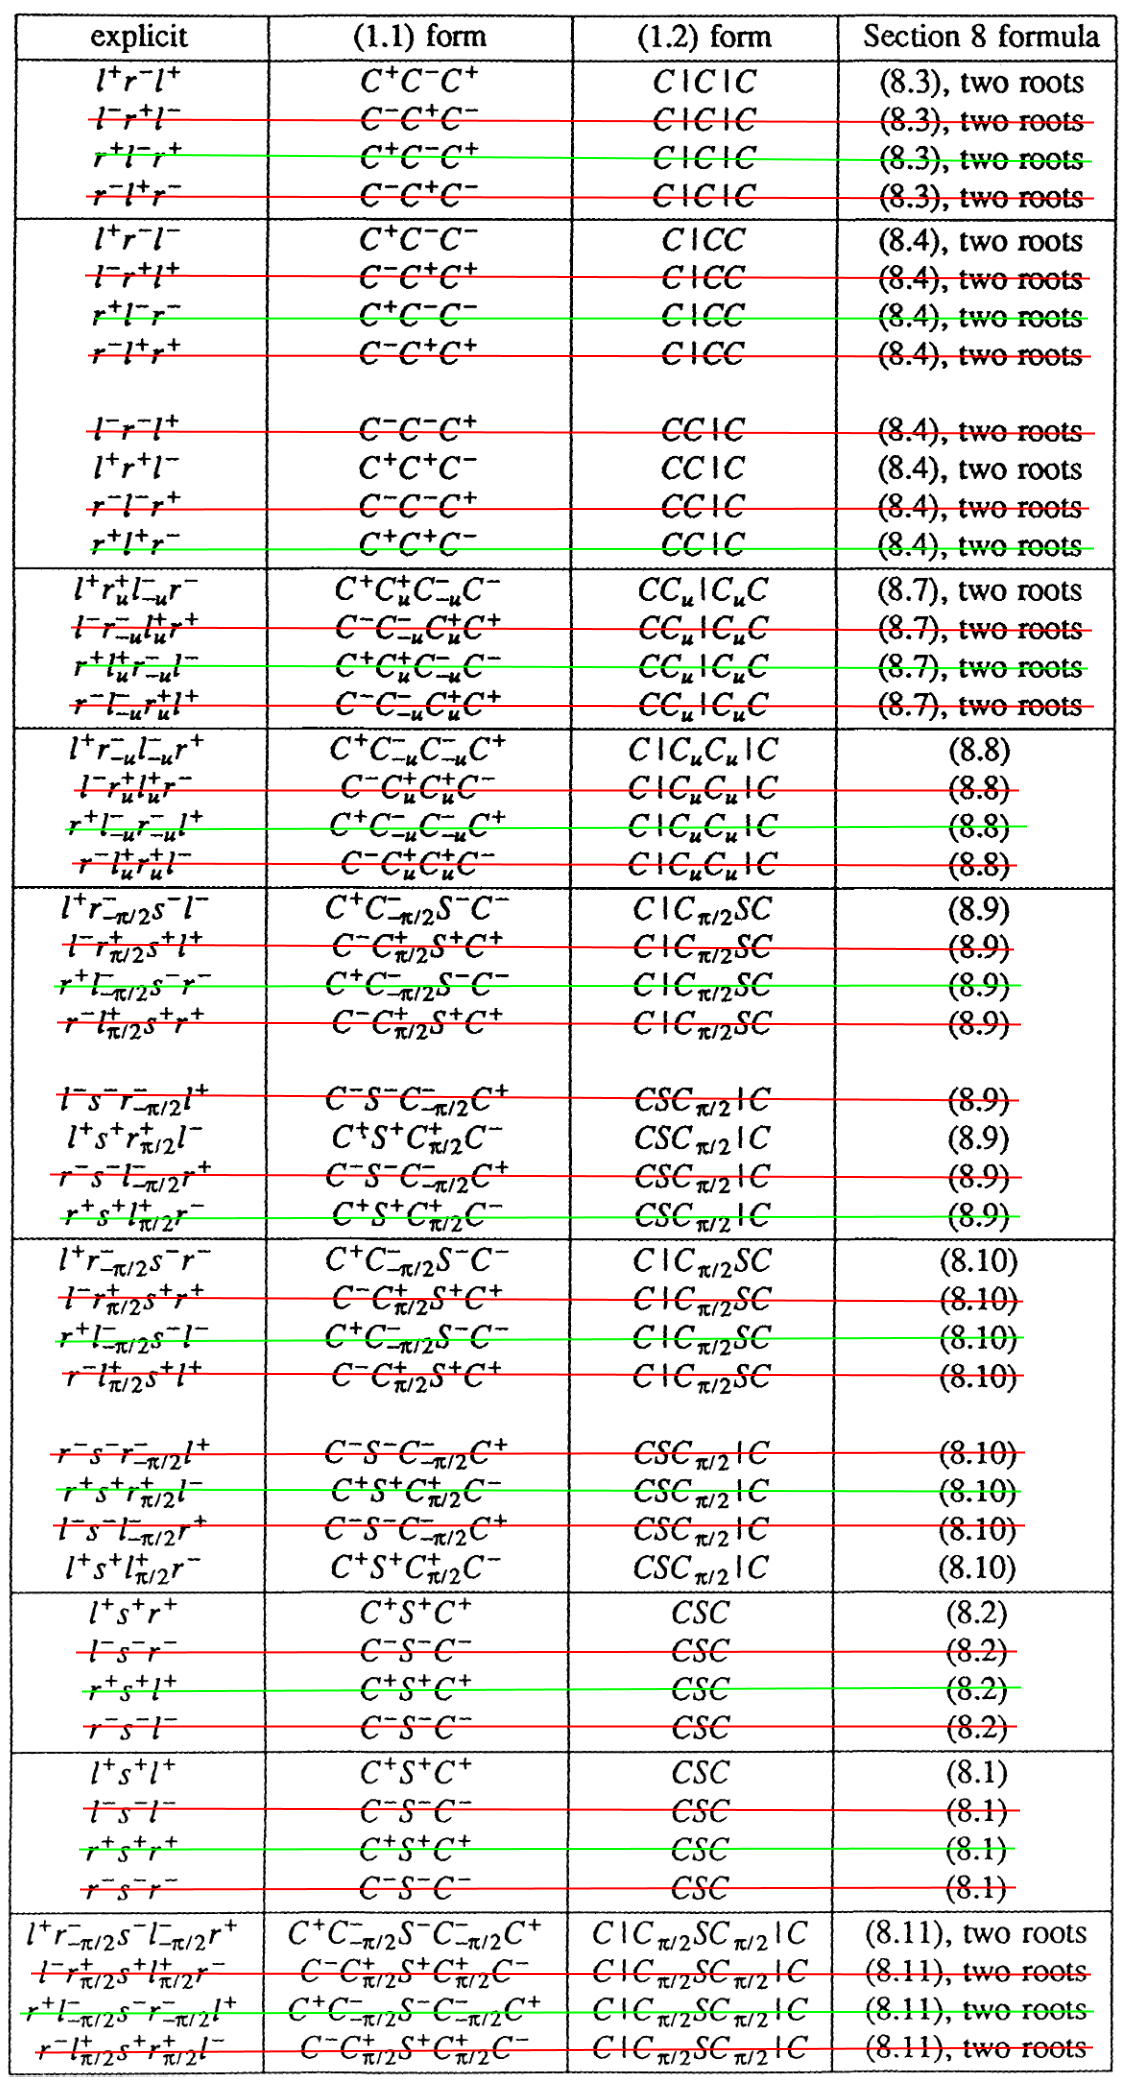
\includegraphics[width=0.4\linewidth]{Illustrations/ReedsSheppPossibilitiesNoTitleNoTimeflipNoReflect.png}
  \caption{All Reeds-Shepp paths with \textcolor{red}{timeflip} and \textcolor{green}{reflect} simplifications}
  \label{fig:sub1}
\end{figure}
\end{frame}

\begin{frame}

\frametitle{Reeds-Shepp paths: reverse simplification}

\begin{figure}
\centering
  \centering
  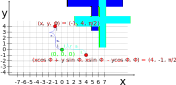
\includegraphics[width=\linewidth]{Illustrations/reverse.png}
  \caption{Reverse simplification: $l^-s^-r^-l^+$ goes from the (0, 0, 0) to ($x, y, \phi$) and $l^+r^-s^-l^-$ goes from (0, 0, 0) to ($x$cos $\phi+y$sin $\phi$, $x$sin $\phi-y$cos $\phi$, \phi)}
  \label{fig:sub1}
\end{figure}
\end{frame}

\begin{frame}

\frametitle{Reeds-Shepp paths: reverse simplification}

\begin{figure}
\centering
  \centering
  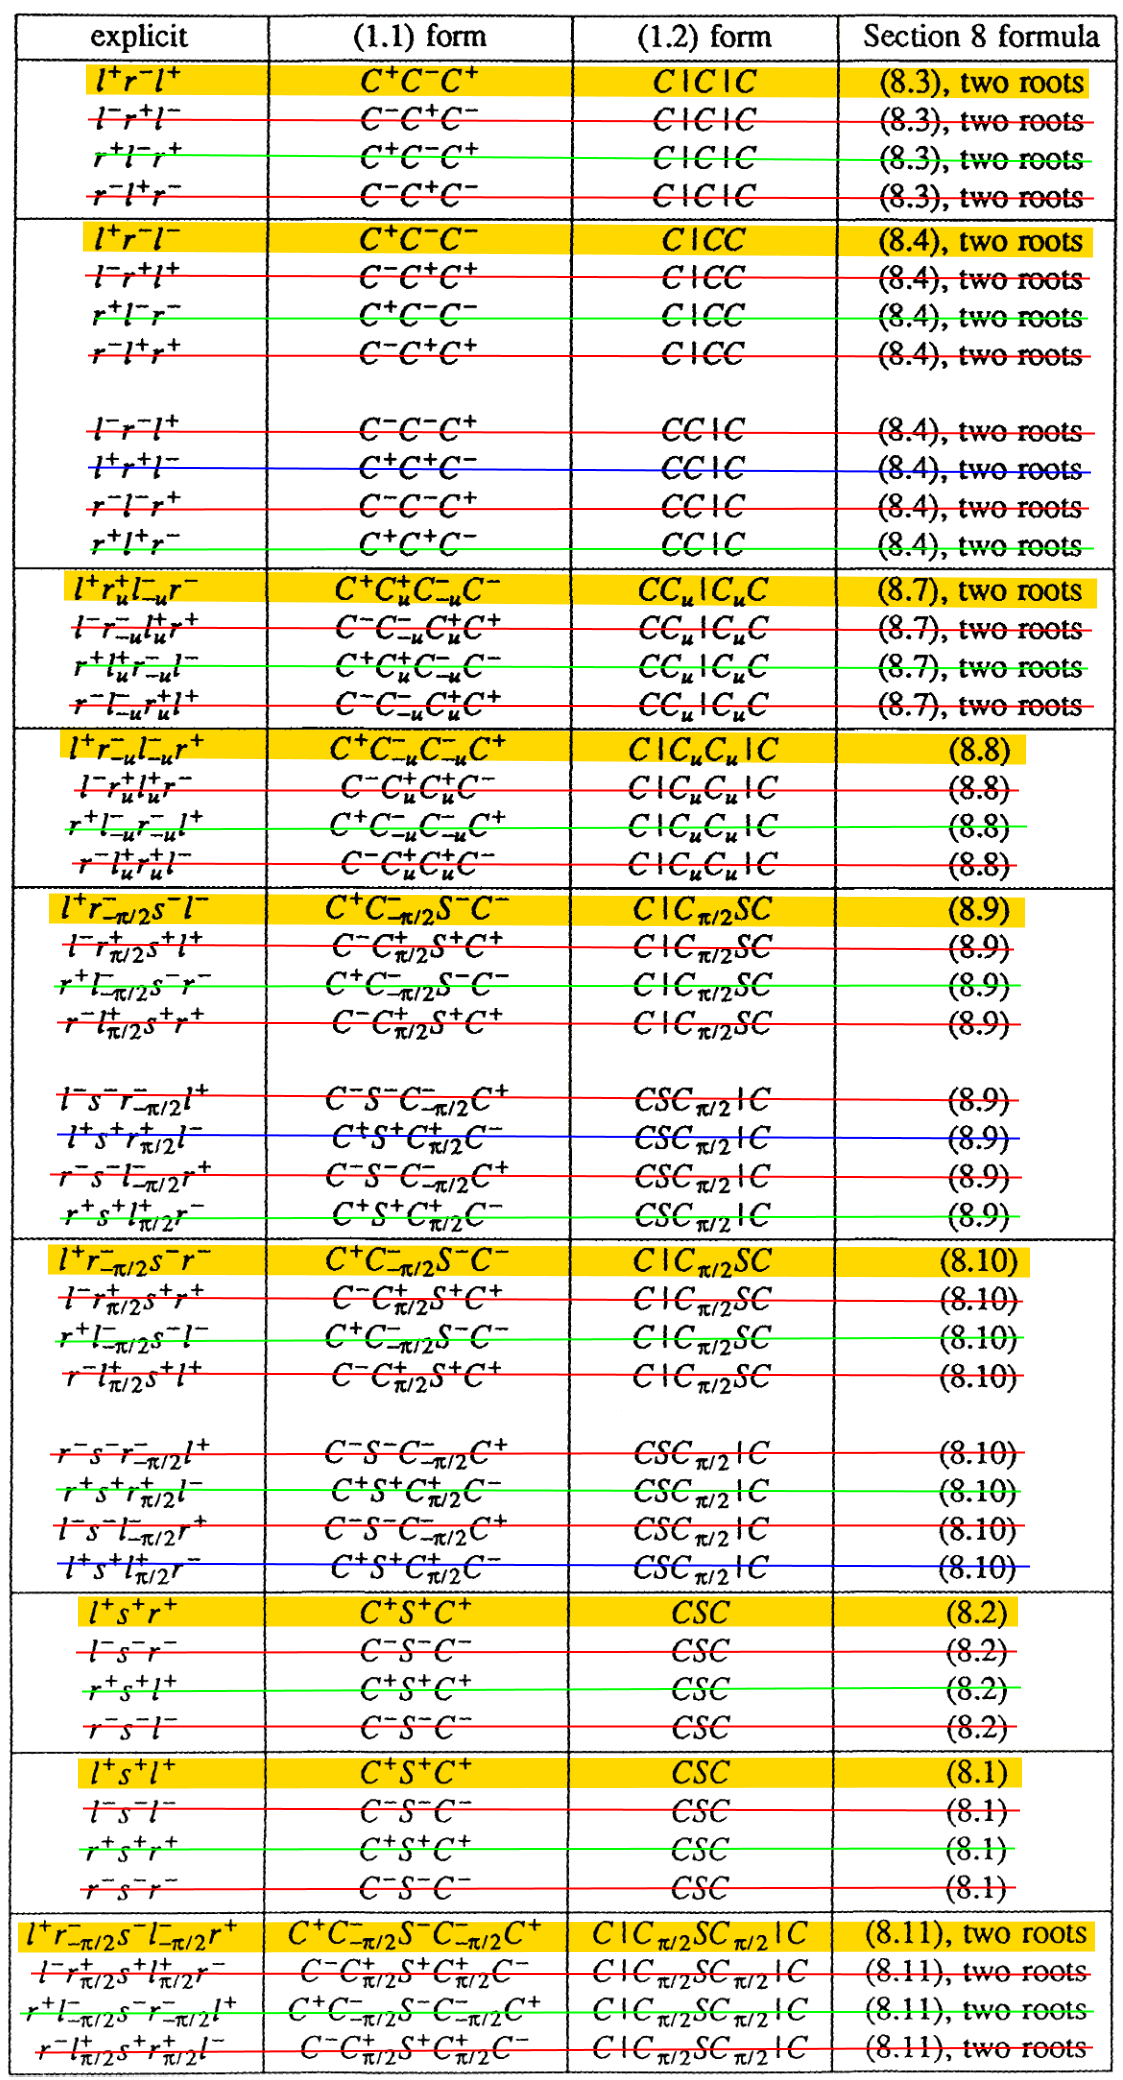
\includegraphics[width=0.4\linewidth]{Illustrations/ReedsSheppPossibilitiesNoTitleNoTimeflipNoReflectNoReverse.png}
  \caption{\textcolor{yellow}{Reeds-Shepp paths} with \textcolor{red}{timeflip}, \textcolor{green}{reflect}, \textcolor{blue}{reverse} simplifications}
  \label{fig:sub1}
\end{figure}
\end{frame}

%\section{Implementation details}

\begin{frame}

\frametitle{Reeds-Shepp paths: case $l_t^+s_u^+l_v^+$}

\begin{itemize}
	\item ($u, t$) := $R$($x$ - sin $\phi$, $y$ - 1 + cos $\phi$)
	\item $v$ := $M(\phi - t)$
	%\item $L = |t| + |u| + |v|$
\end{itemize}

With:

\begin{itemize}
	\item ($r, \theta$) := $R(x, y)$ for the polar transform $r$cos $\theta = x$ and $r$sin $\theta = y$ with $r \leq 0$ and $-\pi \leq \theta < \pi$
	\item $\phi = M(\theta)$ if $\phi \equiv \theta$ mod $2\pi$ and $-\pi \leq \phi < \pi$
\end{itemize}

\end{frame}

\begin{frame}

\frametitle{Dubins and Reeds-Shepp paths in reality}

\begin{itemize}
	\item All kinds of sources for error in the real-world
	\pause
	\item Paths found in the absence of obstacles however can use a rapidly exploring random tree and Dubins' pseudo distance or Reeds-Shepp distance
\end{itemize}

\end{frame}

\begin{frame}

\frametitle{Sources}

	\begin{itemize}
		\item Optimal paths for a car that goes both forwards and backwards (1990), J. A. Reeds and L. A. Shepp
		\item Planning algorithms: Reeds-Shepp curves (2006), Steven M. LaValle
		%\item Planning algorithms: Dubins curves (2006), Steven M. LaValle
		\item A Comprehensive, Step-by-Step Tutorial to Computing Dubins' Paths (2013), Andy G's Blog
	\end{itemize}
\end{frame}

\end{document}